\documentclass[conference]{IEEEtran}
\IEEEoverridecommandlockouts
\usepackage{cite}
\usepackage{amsmath,amssymb}
\usepackage{graphicx}
\usepackage{booktabs}
\usepackage{url}
\usepackage[hidelinks,pdfauthor={},pdfcreator={},pdfproducer={}]{hyperref}
\hypersetup{pdftitle={Masked DeepAR with a Zero-Run Persistence Hurdle: an ML+DL Hybrid for Sparse Retail Demand}}
\graphicspath{{../results/phase2/figures/}{../results/phase2/zero_model/}{../docs/figures/eda/}}

\begin{document}
\title{Masked DeepAR with a Zero-Run Persistence Hurdle:\\an ML+DL Hybrid for Sparse, Partly Censored Retail Demand}
\author{\IEEEauthorblockN{Anonymous Submission}\IEEEauthorblockA{Phase~2 (Deep Learning) project report}}
\maketitle

\begin{abstract}
Daily retail sales are sparse counts, and long runs of zero sales may be stockouts rather than absent demand. In Phase~1 a DeepAR network trained with these runs masked from its loss was a good model of visible demand but under-predicted recorded zeros. The unmasked network showed the reverse trade-off. Phase~2 adds (i) an improved DeepAR with seasonal lags and checkpoint selection on a validation block inside the history, and (ii) a LightGBM \emph{zero-run persistence model} that predicts the probability of a recorded zero at each horizon. The two are joined by a hurdle that takes its zero mass from the ML model and the shape of positive sales from DeepAR. The result is a valid count distribution with exact sampling. On 1,200 M5 series, four rolling 28-day test origins and three seeds, the hybrid has the lowest error on recorded sales of all compared models (WAPE $0.6707\pm0.0003$, mean pinball $0.2533\pm0.0003$). Paired series-bootstrap intervals show it beats masked DeepAR, unmasked DeepAR, LightGBM and the Phase~1 Kalman--LightGBM hybrid on recorded sales, and beats unmasked DeepAR also on days outside long zero runs. Its randomised PIT is flatter than that of masked DeepAR, and a naive zero-inflated fusion is clearly worse. The gain is concentrated in series that are already in a zero run at the origin. On days outside such runs the hybrid is slightly worse than masked DeepAR, and the Phase~1 Kalman--LightGBM model remains the best. M5 has no inventory data, so nothing here is a stockout prediction.
\end{abstract}

\begin{IEEEkeywords}
DeepAR, intermittent demand, hurdle model, negative binomial, zero-inflation, probabilistic forecasting, hybrid ML+DL, M5
\end{IEEEkeywords}

\section{Introduction}
Replenishment needs demand quantiles; the newsvendor optimum is the $C_u/(C_u+C_o)$ quantile. In our M5 subset 59\% of available item-days record zero sales and 90\% of series are intermittent or lumpy. Some long zero runs are probably stockouts, but M5 contains no inventory records, so they can only be flagged heuristically (Section~\ref{sec:data}).

Phase~1 compared Kalman filtering, LightGBM, a Kalman--LightGBM hybrid and DeepAR~\cite{salinas2020} under a leak-safe rolling-origin protocol. Its ablation showed a trade-off. DeepAR with the loss masked on flagged days scored better on non-flagged days. Without the mask, it scored better on all recorded days, because it learned the long zero runs as demand. Phase~2 asks: \emph{can a separately trained, calibrated model of zero-run persistence supply the recorded zeros, while DeepAR stays a model of demand, and does this beat simply not masking?}

Contributions: (1) a DeepAR v2 with seasonal lags and a history validation block with best-checkpoint restore, selected on a validation origin only; (2) a causal zero-run persistence model with non-learned baselines, including a Kaplan--Meier renewal model; (3) a Rao-Blackwellised hurdle fusion of the two with exact sampling, and alternative fusions as ablations; (4) evaluation over three seeds with series-level paired bootstrap, randomised PIT and zero-mass calibration, including the slices where the hybrid fails.

\section{Related Work}
\textbf{Deep forecasters.} LSTMs~\cite{hochreiter1997} trained globally across series are competitive when inputs are scaled and seasonality is presented explicitly~\cite{hewamalage2021,bandara2020}. DeepAR~\cite{salinas2020} fits an autoregressive LSTM with a parametric likelihood and forecasts by ancestral sampling. MQ-RNN~\cite{wen2017mqrnn} and Temporal Fusion Transformers~\cite{lim2021} output quantiles directly; they give no count pmf, which our fusion needs.

\textbf{Intermittent demand.} Croston separates demand sizes and intervals~\cite{croston1972}; its bias and the SBA correction are analysed in~\cite{syntetos2005accuracy}, and TSB handles obsolescence~\cite{teunter2011}. Deep renewal processes~\cite{turkmen2021} make both parts neural and probabilistic, and~\cite{jeon2022} propose a robust RNN for intermittent series.

\textbf{Zero-inflated and hurdle models.} Zero-inflated models~\cite{lambert1992} mix an extra ``always zero'' state with a count distribution, so zeros come from two sources. Hurdle models~\cite{mullahy1986} use one binary process for zero vs.\ positive and a zero-truncated count model for positive values. This distinction drives our fusion (Section~\ref{sec:fusion}).

\textbf{Hybrids.} ES-RNN~\cite{smyl2020}, deep state-space models~\cite{rangapuram2018} and Deep Factors~\cite{wang2019deepfactors} give statistical and neural parts different roles inside one model, rather than averaging outputs. Our Phase~1 Kalman--LightGBM is a feature-level ML+ML hybrid; the Phase~2 hybrid combines ML and DL at the level of the predictive distribution.

\textbf{Evaluation.} We follow the calibration--sharpness paradigm~\cite{gneiting2007calibration} with proper scores~\cite{gneiting2007}, use the randomised PIT for counts~\cite{czado2009}, heed the pitfalls of point metrics for retail counts~\cite{kolassa2016}, and resample whole series to respect dependence~\cite{kunsch1989}. With only four origins, a Diebold--Mariano test~\cite{diebold1995} across time is not informative, so we report per-origin signs instead.

\section{Data, Censoring Assumptions and Protocol}\label{sec:data}
\textbf{Data.} 400 items from each of the stores CA\_1, TX\_1 and WI\_1 of M5~\cite{makridakis2022accuracy}, the last 1,000 days (2013-08-27 to 2016-05-22), a frozen stratified subset. A day is \emph{available} if the item has a posted price that week and is past its first sale. Covariates: 13 calendar, 5 event, SNAP and 4 price features; M5 publishes prices in advance, so they are treated as known.

\textbf{Observed vs.\ latent.} We observe recorded sales $y_{it}$ and availability; latent demand $d_{it}$ and stock status are unobserved. Assumption A1: $y=d$ when in stock and $y=0$ otherwise. A zero run of length $L$ in a series with $\geq10$ sales is \emph{flagged} by the proxy if $L\ge\max(28,3\,\mathrm{ADI})$. The proxy is a heuristic. It produces false positives (quiet periods, delisting) and false negatives (short or partial outages).

\textbf{Protocol.} Four test origins (2016-01-31 to 2016-04-24, step 28), horizon $H=28$, seven quantile levels. The context passed to a model is cut at the origin, and the proxy is recomputed on the history slice. One earlier origin (2016-01-03) is used only for design selection. Inside each fit the last $H$ days of history form a validation block. 84 series (7\%) are \emph{simulated} cold-start series: their history is hidden, and they are not real launches. We evaluate 1,116 warm series on (a) \emph{all days} (124,992 cells, recorded sales) and (b) \emph{non-censored} days (114,127 cells, excluding days flagged in hindsight), as a proxy view of visible demand.

\section{Methods}
\subsection{DeepAR v2 (DL component)}
A 2-layer, 64-unit LSTM is shared across series. Its input at step $t$ is
$[\,y_{t-1},y_{t-7},y_{t-14},y_{t-28}]/\nu$ with an observed-flag for each lag, $\log\nu$, the covariates of day $t$, and embeddings of item (8-d) and dept/category/store/state (4-d). The scale is $\nu=1+\bar y_{\text{context}}$. The output is a negative binomial
\begin{equation}
\mathrm{NB}(y;\mu,\alpha)=\tfrac{\Gamma(y+r)}{\Gamma(r)\,y!}\big(\tfrac{r}{r+\mu}\big)^{r}\big(\tfrac{\mu}{r+\mu}\big)^{y},\ r=\alpha^{-1},
\end{equation}
with $\mu=\nu\,\mathrm{softplus}(w_\mu^\top h_t)$, $\alpha=\mathrm{softplus}(w_\alpha^\top h_t)/\sqrt\nu$, $\mathbb E y=\mu$ and $\mathrm{Var}\,y=\mu+\alpha\mu^2$. The NLL is averaged over available, unflagged targets only. Masked days enter the input as $(0,\text{flag}=0)$, so masked DeepAR models demand \emph{given normal selling}. In sampling, a lag $y_{T+h-k}$ is observed if $h\le k$ and is otherwise taken from the same sample path. Training: windows of 84+28 days from the last 730 days, batch 128, Adam ($10^{-3}$, cosine to $10^{-4}$), L2 $10^{-5}$, gradient clip 10, dropout 0.1, item-id dropout 0.15, 2,500 steps at the first origin and 800 warm-started steps later. \emph{Validation}: training windows end before the last 28 days of history; every 100 steps the NLL on that block is computed, and the best checkpoint is restored (patience 5)~\cite{prechelt1998}. At warm-started origins the incoming weights compete as step 0. AdamW~\cite{loshchilov2019} and a causal age feature are implemented as options.

\textbf{Selection (validation origin only).} Table~\ref{tab:e02} shows the design ladder, ranked by a rule fixed before the runs. Lags gave the only clear gain. Age and AdamW fell inside a 0.5\% tie band and were not adopted. Early stopping never triggered, because the step budget, not over-fitting, was binding (Fig.~\ref{fig:curves}).
\begin{table}[t]
\caption{DeepAR design selection on the \emph{validation} origin 2016-01-03 (E02). Rule fixed in advance: lowest non-censored pinball; gaps $<0.5\%$ go to the simpler model.}
\label{tab:e02}
\centering
\footnotesize
\resizebox{\columnwidth}{!}{\begin{tabular}{@{}lcccr@{}}
\toprule
Variant & WAPE & Pinball & Pinball$_{nc}$ & best step\\
\midrule
Phase 1 DeepAR & 0.7305 & 0.2552 & 0.2750 & --\\
+ validation checkpoint & 0.7290 & 0.2557 & 0.2768 & 2300\\
+ lags 7/14/28 (selected) & 0.7311 & 0.2550 & 0.2728 & 2100\\
+ age & 0.7324 & 0.2550 & 0.2722 & 2500\\
+ AdamW (wd 0.01) & 0.7330 & 0.2549 & 0.2721 & 2500\\
\bottomrule
\end{tabular}}
\end{table}


\subsection{Zero-run persistence model (ML component)}
Target: $\pi_h(T)=P(y_{T+h}=0\mid\mathcal F_T)$ on available days. It concerns \emph{recorded} zeros, is observable, needs no inventory labels and is not a stockout probability. Features at anchor $t$, all causal: the current zero-run length $r_t$, $r_t/\mathrm{ADI}_t$, the causal proxy flag, completed-run statistics up to $t$ (count, mean, max, number $\ge$28 days), expanding ADI, rolling non-zero rates and means (7--112 days), lags, covariates of the target day, hierarchy codes and $h$. A single LightGBM~\cite{ke2017} binary model with log loss covers all horizons. Training rows use anchors every 7 days with $t+h\le T-H$ (at most 600k rows). Validation rows use anchor $T-H$, and early stopping is applied on them. No class re-weighting is used, because re-weighting would distort the probabilities the fusion consumes. Baselines: series zero rate, last-28-day zero rate, and a Kaplan--Meier~\cite{kaplan1958} renewal model. The renewal model pools run durations by ADI quartile and treats the open run as right-censored: $\pi_h^{\mathrm{KM}}=s_h+(1-s_h)z_i$ with $s_h=S(r+h-1)/S(r-1)$.

\subsection{Hurdle fusion}\label{sec:fusion}
DeepAR's marginal at horizon $h$ is a mixture over $S=200$ paths, $p_D(y)=\frac1S\sum_s\mathrm{NB}(y;\mu_s,\alpha_s)$, with exact zero mass $p_D(0)=\frac1S\sum_s (r_s/(r_s+\mu_s))^{r_s}$. The hybrid is
\begin{equation}
q(0)=\pi_h,\qquad q(y)=(1-\pi_h)\,\frac{p_D(y)}{1-p_D(0)},\quad y\ge1.
\end{equation}
It is a valid pmf on $\mathbb N_0$, and $\mathbb E_q y=(1-\pi_h)\sum_s\mu_s/\sum_s(1-p_{0,s})$. Its quantiles are $Q(\tau)=0$ for $\tau\le\pi_h$ and $F_+^{-1}((\tau-\pi_h)/(1-\pi_h))$ otherwise. Positive draws are exact: choose path $s$ with probability $\propto 1-p_{0,s}$, then invert the zero-truncated NB. The naive zero-inflated mixture $\pi\delta_0+(1-\pi)p_D$ has $q(0)=\pi+(1-\pi)p_D(0)>\pi$. Because $\pi$ is trained on the event $y=0$ itself, this counts DeepAR's zeros twice. Ablations change only $q(0)$: \texttt{zi\_naive}; \texttt{zi\_inflate} $q(0)=\max(\pi,p_D(0))$; \texttt{gated}, which uses $\pi$ only for series flagged at the origin. A no-DL variant replaces $p_D(\cdot\mid y>0)$ by the empirical distribution of the series' positive sales over the last 112 days. Fig.~\ref{fig:arch} shows the architecture.

\begin{figure}[t]\centering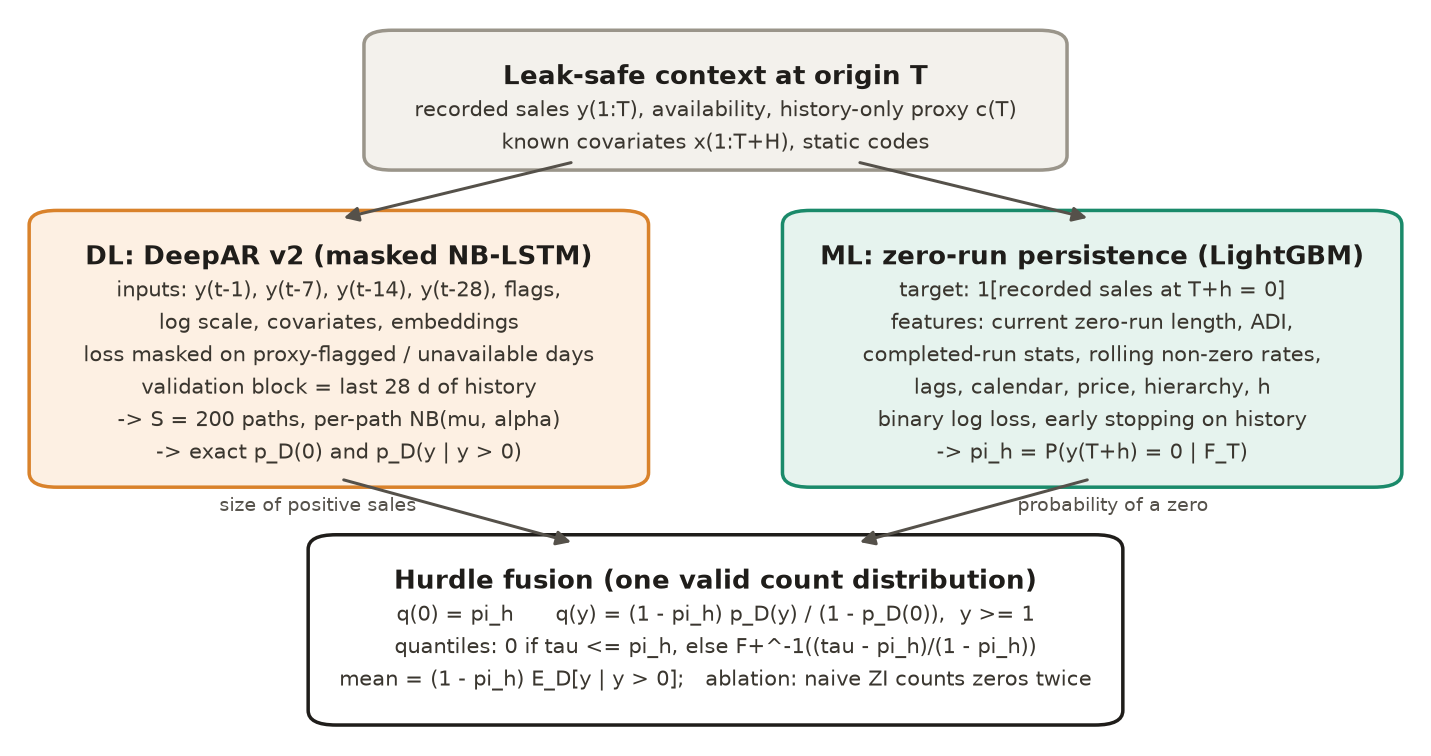
\includegraphics[width=\columnwidth]{hybrid_architecture.png}
\caption{Hybrid: the ML model gives the probability of a recorded zero; masked DeepAR gives the size distribution of positive sales.}\label{fig:arch}\end{figure}

\subsection{Leakage controls and tests}
65 automated tests pass (35 from Phase~1, 30 new). They check: the NB NLL against \texttt{scipy} ($<10^{-8}$); sampler mean, variance and $P(0)$; masked-loss accounting; that training windows avoid the validation block; that DeepAR, the zero-run features and the zero model are bit-identical after the data after the origin are perturbed; same-seed reproducibility; Kaplan--Meier with censoring; hurdle pmf, quantiles and the truncated sampler against closed forms; uniformity of the randomised PIT under a correct model; and an end-to-end pipeline run of the hybrid on a synthetic fixture. Re-running Phase~1 DeepAR with the Phase~2 code reproduced all 1,075,200 forecast values exactly.

\section{Results}
\subsection{Zero-run persistence model on its own}
Table~\ref{tab:zero} scores $P(y=0)$ on the test cells. The LightGBM model beats every non-learned baseline. Paired series bootstrap of the Brier difference: $-0.0146$ $[-0.0169,-0.0126]$ vs.\ Kaplan--Meier and $-0.0168$ vs.\ the series zero rate. It also beats the zero mass of masked DeepAR v2 ($-0.0079$ $[-0.0102,-0.0058]$), most strongly inside long runs (Brier 0.101 vs.\ 0.172). It is only tied with \emph{unmasked} DeepAR ($-0.0007$ $[-0.0015,+0.0000]$). Removing the explicit run-length features changes nothing measurable ($-0.0002$ $[-0.0006,+0.0002]$): rolling non-zero rates carry the same information.
\begin{table}[t]
\caption{Zero-run persistence model (E04): scores of $P(y_{T+h}=0)$ on the test cells of warm series. ECE: 10-bin expected calibration error.}
\label{tab:zero}
\centering
\footnotesize
\resizebox{\columnwidth}{!}{\begin{tabular}{@{}lcccc|cc@{}}
\toprule
& \multicolumn{4}{c|}{All warm cells (124,992)} & \multicolumn{2}{c}{Run $\ge$28 d at origin}\\
Predictor & Brier & Log loss & ECE & AUC & Brier & Log loss\\
\midrule
Series zero rate & 0.1915 & 0.5643 & 0.0329 & 0.774 & 0.1387 & 0.4385\\
Zero rate, last 28 d & 0.1843 & 0.6778 & 0.0393 & 0.792 & 0.1326 & 1.8325\\
Kaplan--Meier renewal & 0.1893 & 0.5710 & 0.0684 & 0.789 & 0.1114 & 0.4805\\
\textbf{LightGBM zero model} & 0.1746 & 0.5229 & 0.0075 & 0.810 & 0.1013 & 0.3437\\
\quad without run features & 0.1748 & 0.5235 & 0.0080 & 0.809 & 0.1014 & 0.3451\\
DeepAR P1 $p_D(0)$ & 0.1850 & 0.5497 & 0.0341 & 0.788 & 0.2018 & 0.6026\\
DeepAR v2 $p_D(0)$ & 0.1826 & 0.5442 & 0.0259 & 0.792 & 0.1723 & 0.5355\\
DeepAR v2 unmasked $p_D(0)$ & 0.1754 & 0.5255 & 0.0066 & 0.808 & 0.1024 & 0.3543\\
\bottomrule
\end{tabular}}
\end{table}


\subsection{Main comparison}
Table~\ref{tab:main2} gives all models, and Table~\ref{tab:seeds} the seed spread. On recorded sales the hybrid is best on WAPE and pinball loss. Its seed standard deviation (0.0003) is far below the gaps to the other models. On non-censored days it does not lead: the Phase~1 Kalman--LightGBM model is best there.
\begin{table*}[t]
\caption{Test results, 4 origins $\times$ 28 days. All days: 124,992 cells (recorded sales); non-censored: 114,127 cells; simulated cold start: 9,408 cells. $^{\dagger}$mean over seeds 42, 43, 44 (sd in Table~\ref{tab:seeds}); other Phase~2 rows seed 42. Lower is better except coverage (nominal 0.80/0.90).}
\label{tab:main2}
\centering
\resizebox{\textwidth}{!}{\begin{tabular}{@{}lcccccccc@{}}
\toprule
& \multicolumn{4}{c}{All days} & \multicolumn{2}{c}{Non-censored} & \multicolumn{2}{c}{Cold start}\\
\cmidrule(lr){2-5}\cmidrule(lr){6-7}\cmidrule(l){8-9}
Model & WAPE & Pinball & Cov80 & Cov90 & WAPE & Pinball & WAPE & Pinball\\
\midrule
Seasonal naive (4 wk) & 0.7724 & 0.2899 & 0.838 & 0.914 & 0.7591 & 0.3092 & 0.8746 & 0.3188\\
Kalman (local) & 0.7226 & 0.2736 & 0.831 & 0.914 & 0.6860 & 0.2822 & 0.8385 & 0.3226\\
LightGBM & 0.7094 & 0.2637 & 0.871 & 0.941 & 0.6630 & 0.2707 & 0.7733 & 0.2736\\
Kalman--LightGBM (P1 hybrid) & 0.7039 & 0.2620 & 0.875 & 0.940 & \textbf{0.6598} & \textbf{0.2693} & 0.7604 & 0.2748\\
Ensemble P1 (K, L, DeepAR P1) & 0.7030 & 0.2623 & 0.827 & 0.919 & 0.6647 & 0.2706 & 0.7828 & 0.2832\\
Ensemble P2 (K, L, DeepAR v2) & 0.7008 & 0.2616 & 0.826 & 0.919 & 0.6646 & 0.2705 & 0.7751 & 0.2805\\
DeepAR P1$^{\dagger}$ & 0.6948 & 0.2612 & 0.930 & 0.964 & 0.6644 & 0.2721 & 0.7671 & 0.2766\\
DeepAR v2$^{\dagger}$ & 0.6913 & 0.2606 & 0.930 & 0.964 & 0.6634 & 0.2720 & 0.7534 & 0.2733\\
DeepAR v2, unmasked$^{\dagger}$ & 0.6783 & 0.2567 & 0.927 & 0.962 & 0.6709 & 0.2764 & 0.7616 & 0.2754\\
Zero model + empirical sizes & 0.6876 & 0.2609 & 0.929 & 0.962 & 0.6816 & 0.2817 & \textbf{0.7407} & 0.2740\\
\textbf{Hybrid (DeepAR v2 + zero model)}$^{\dagger}$ & \textbf{0.6707} & \textbf{0.2533} & 0.931 & 0.964 & 0.6644 & 0.2734 & 0.7538 & \textbf{0.2721}\\
\bottomrule
\end{tabular}}
\end{table*}

\begin{table}[t]
\caption{Seed variability: mean $\pm$ sd over seeds 42, 43, 44 (warm series).}
\label{tab:seeds}
\centering
\footnotesize
\resizebox{\columnwidth}{!}{\begin{tabular}{@{}lcccc@{}}
\toprule
& \multicolumn{2}{c}{All days} & \multicolumn{2}{c}{Non-censored}\\
\cmidrule(lr){2-3}\cmidrule(l){4-5}
Model & WAPE & Pinball & WAPE & Pinball\\
\midrule
DeepAR P1 & 0.6948$\pm$0.0025 & 0.2612$\pm$0.0007 & 0.6644$\pm$0.0011 & 0.2721$\pm$0.0003\\
DeepAR v2 & 0.6913$\pm$0.0012 & 0.2606$\pm$0.0004 & 0.6634$\pm$0.0006 & 0.2720$\pm$0.0006\\
DeepAR v2, unmasked & 0.6783$\pm$0.0023 & 0.2567$\pm$0.0012 & 0.6709$\pm$0.0025 & 0.2764$\pm$0.0013\\
Hybrid & 0.6707$\pm$0.0003 & 0.2533$\pm$0.0003 & 0.6644$\pm$0.0003 & 0.2734$\pm$0.0003\\
\bottomrule
\end{tabular}}
\end{table}


\subsection{Ablations and pairwise tests}
Table~\ref{tab:abl2} answers one question per row.
\emph{DeepAR v2 vs.\ P1:} WAPE improves significantly ($-0.0035$ $[-0.0057,-0.0016]$, 4/4 origins). Pinball loss does not ($-0.0006$ $[-0.0013,+0.0001]$), so the DL changes are minor.
\emph{Masking:} unmasked DeepAR is better on all days and worse on non-censored days, both significantly, which replicates the Phase~1 trade-off over three seeds.
\emph{Persistence component:} the hybrid improves on DeepAR by $-0.0073$ pinball on all days (4/4 origins). On non-censored days it is worse by $+0.0013$ $[+0.0002,+0.0027]$.
\emph{Versus simply not masking:} the hybrid beats unmasked DeepAR on \emph{both} views ($-0.0034$ and $-0.0030$, 4/4 origins). This is the main evidence that the hybrid adds value beyond the masking choice.
\emph{DL component:} replacing DeepAR's positive part by empirical sizes costs $+0.0072$ (all days) and $+0.0079$ (non-censored).
\emph{Fusion:} naive ZI is much worse ($+0.0224$), inflate-only ZI and gating are slightly worse. The hurdle is therefore the best of the tested fusions.
\emph{Ensemble:} an equal-weight average of Kalman, LightGBM and DeepAR v2 is not better than DeepAR v2 on all days.
\begin{table*}[t]
\caption{Ablations and pairwise comparisons on mean pinball loss. $\Delta$ = changed $-$ baseline (negative: change helps); 95\% paired-bootstrap CI over series (1,000 draws); * = CI excludes 0; ``orig.'' = number of the 4 origins on which the change helps.}
\label{tab:abl2}
\centering
\footnotesize
\resizebox{\textwidth}{!}{\begin{tabular}{@{}llrrlrrlr@{}}
\toprule
& & \multicolumn{3}{c}{All days} & \multicolumn{3}{c}{Non-censored} & \\
\cmidrule(lr){3-5}\cmidrule(lr){6-8}
Experiment & Unit & Value & $\Delta$ & 95\% CI & Value & $\Delta$ & 95\% CI & orig.\\
\midrule
DeepAR P2 vs P1 & 3 seeds & 0.2606 & -0.0006 & [-0.0013, +0.0001] & 0.2720 & -0.0000 & [-0.0005, +0.0004] & 3/4\\
Loss masking (DeepAR) & 3 seeds & 0.2567 & -0.0039* & [-0.0064, -0.0014] & 0.2764 & +0.0043* & [+0.0028, +0.0061] & 4/4\\
Hybrid vs DeepAR & 3 seeds & 0.2533 & -0.0073* & [-0.0101, -0.0047] & 0.2734 & +0.0013* & [+0.0002, +0.0027] & 4/4\\
Hybrid vs unmasked DeepAR & 3 seeds & 0.2533 & -0.0034* & [-0.0048, -0.0022] & 0.2734 & -0.0030* & [-0.0042, -0.0019] & 4/4\\
Hybrid vs LightGBM & 3 seeds vs 1 & 0.2533 & -0.0103* & [-0.0139, -0.0071] & 0.2734 & +0.0027 & [-0.0001, +0.0051] & 4/4\\
Hybrid vs Kalman-LightGBM & 3 seeds vs 1 & 0.2533 & -0.0087* & [-0.0131, -0.0050] & 0.2734 & +0.0041* & [+0.0014, +0.0065] & 4/4\\
Kalman-LightGBM vs LightGBM & single & 0.2620 & -0.0017* & [-0.0028, -0.0001] & 0.2693 & -0.0014* & [-0.0019, -0.0010] & 4/4\\
No DL component & seed 42 & 0.2609 & +0.0072* & [+0.0046, +0.0108] & 0.2817 & +0.0079* & [+0.0051, +0.0121] & 0/4\\
Fusion: naive ZI & seed 42 & 0.2761 & +0.0224* & [+0.0212, +0.0235] & 0.3000 & +0.0263* & [+0.0251, +0.0274] & 0/4\\
Fusion: inflate-only ZI & seed 42 & 0.2544 & +0.0007* & [+0.0004, +0.0010] & 0.2747 & +0.0009* & [+0.0006, +0.0013] & 0/4\\
Fusion: gated & seed 42 & 0.2553 & +0.0016* & [+0.0004, +0.0028] & 0.2734 & -0.0003 & [-0.0011, +0.0004] & 1/4\\
Ensemble P2 vs DeepAR v2 & seed 42 & 0.2616 & +0.0012 & [-0.0013, +0.0038] & 0.2705 & -0.0022* & [-0.0044, -0.0002] & 1/4\\
\bottomrule
\end{tabular}}
\end{table*}


\subsection{Calibration and failure cases}
The randomised PIT (Fig.~\ref{fig:pit}) of masked DeepAR has too much mass in the lowest bins, because it predicts too few zeros. The hybrid's histogram is flatter: maximum deviation 0.056--0.084 over seeds, against 0.103--0.114 for masked DeepAR (Table~\ref{tab:calib}). Its implied $q(0)$ has the lowest Brier score of all models. The naive ZI fusion over-predicts zeros (ECE 0.171). All DeepAR-based models over-cover the 80/90\% intervals (about 0.93/0.96), so we do not claim the quantiles are calibrated overall.
Table~\ref{tab:slices2} locates the effect. For series in a zero run of $\ge$28 days at the origin (7.9\% of series-origins), the hybrid improves pinball by $-0.062$ on all days but worsens it by $+0.064$ on non-censored days. These are the days on which sales resumed inside the forecast window. In other words, the hybrid forecasts recorded sales, and masked DeepAR remains the better latent-demand model for these series.
\begin{table}[t]
\caption{Calibration of the full predictive distributions (seed 42, warm series, all days): Brier score and ECE of the implied $q(0)$, and the maximum deviation of the randomised-PIT histogram from uniform (10 bins; 0 = flat).}
\label{tab:calib}
\centering
\footnotesize
\resizebox{\columnwidth}{!}{\begin{tabular}{@{}lccc@{}}
\toprule
Model & Brier $q(0)$ & ECE $q(0)$ & PIT max dev.\\
\midrule
deepar\_p1 & 0.1850 & 0.0341 & 0.115\\
deepar\_v2 & 0.1826 & 0.0259 & 0.103\\
deepar\_v2\_nomask & 0.1754 & 0.0066 & 0.050\\
hybrid & 0.1746 & 0.0075 & 0.069\\
hyb\_zi\_naive & 0.2081 & 0.1713 & 1.034\\
hyb\_zi\_inflate & 0.1754 & 0.0237 & 0.122\\
hyb\_gated & 0.1770 & 0.0155 & 0.056\\
hyb\_no\_dl & 0.1746 & 0.0075 & 0.078\\
\bottomrule
\end{tabular}}
\end{table}

\begin{table}[t]
\caption{Hybrid minus DeepAR v2 (3 seeds each), mean pinball, by the causal zero-run state at the origin and by demand class. * = 95\% CI excludes 0.}
\label{tab:slices2}
\centering
\footnotesize
\resizebox{\columnwidth}{!}{\begin{tabular}{@{}lrrr@{}}
\toprule
Slice & series & $\Delta$ all days & $\Delta$ non-cens.\\
\midrule
zero run at origin 0 & 878 & -0.0013 & -0.0009\\
zero run at origin 1-6 & 794 & -0.0013* & -0.0010\\
zero run at origin 7-27 & 341 & -0.0120* & +0.0034*\\
zero run at origin $\ge$28 & 185 & -0.0618* & +0.0636*\\
class: intermittent & 839 & -0.0046* & +0.0007\\
class: lumpy & 162 & -0.0121* & +0.0019\\
class: smooth & 87 & -0.0101 & +0.0021\\
class: erratic & 27 & -0.0526 & +0.0157\\
\bottomrule
\end{tabular}}
\end{table}

\begin{figure}[t]\centering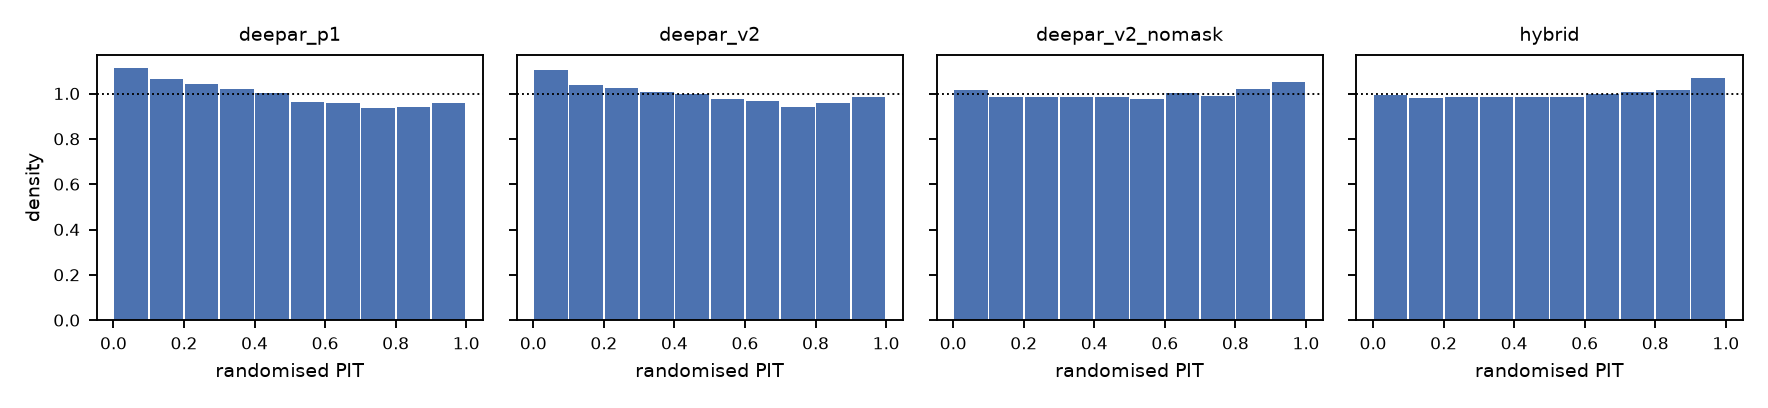
\includegraphics[width=\columnwidth]{pit_histograms.png}
\caption{Randomised PIT, seed 42 (flat = calibrated).}\label{fig:pit}\end{figure}
\begin{figure}[t]\centering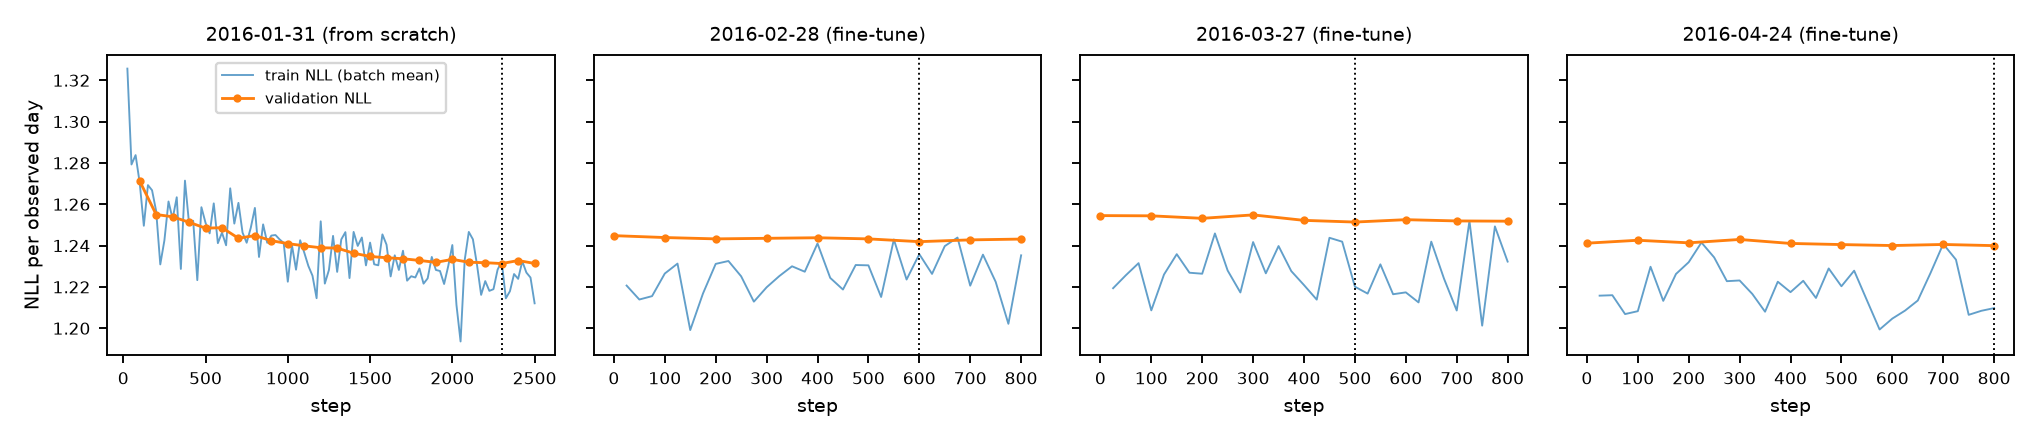
\includegraphics[width=\columnwidth]{training_curves_deepar_v2.png}
\caption{DeepAR v2 train vs.\ validation NLL per origin (seed 42); dotted: restored checkpoint.}\label{fig:curves}\end{figure}

\section{Discussion and Limitations}
\textbf{Is the hybrid meaningful?} The two components have different jobs: a binary, state-dependent zero process and a shared size distribution. The fusion is a valid distribution with exact sampling. Each component was validated alone, and the component ablations show that both contribute: removing either one, or using the naive ZI form, is significantly worse. The value is real but conditional. It appears on recorded sales and in series already in zero runs. On visible demand it is negative against masked DeepAR, and the hybrid does not beat Kalman--LightGBM there.

\textbf{Limitations.} (i) No inventory data: the proxy decides both the masked training days and the non-censored view. (ii) One retailer, three stores, four origins in early 2016; the confidence intervals reflect variation across series, not across time periods. (iii) The main DL comparisons use three seeds, the ablations one seed. (iv) Hyper-parameters are not tuned. DeepAR was selected on one validation origin. (v) The cold start is simulated. (vi) Five planned seed-42 ablations (RB control, no-persistence features inside the hybrid, hybrid on unmasked or Phase~1 DeepAR, DeepAR lag/checkpoint/age/AdamW leave-one-out on test) were \emph{stopped before completion} to limit compute and are not reported. (vii) The Phase~1 Kalman--LightGBM estimates its noise parameters once per origin, so its training anchors use parameters fitted on data up to the origin (training-time look-ahead inside the history).

\textbf{Future work.} Learn $\pi_h$ and the size distribution jointly; replace the proxy with inventory data where available; compare with TFT and deep renewal processes; recalibrate DeepAR's over-wide intervals on the validation origin.

\section{Conclusion}
Joining a masked DeepAR with a calibrated LightGBM model of zero-run persistence through a hurdle gives the most accurate forecasts of recorded sales in this study, with flatter PIT than masked DeepAR. It is better than letting DeepAR learn the zeros itself, and the result is stable over three seeds and four origins. The gain comes from series in long zero runs and costs a little accuracy on visible demand, so the choice between the hybrid and masked DeepAR depends on whether recorded sales or latent demand is the target.

\section*{Reproducibility}
Every table is generated from \texttt{results/phase2/*.csv} by \texttt{scripts/phase2\_tex\_tables.py}. The runs are listed in \texttt{docs/PHASE2\_EXPERIMENT\_LEDGER.md}, and the commands in \texttt{docs/PHASE2\_REPRODUCE.md}.

\bibliographystyle{IEEEtran}
\bibliography{references}
\end{document}
